\documentclass[12pt]{article}
\usepackage[utf8]{inputenc}
\usepackage[russian]{babel}
\usepackage{amssymb,amsmath}
\usepackage{amsmath}
\usepackage{amsthm}
\usepackage{hyperref}
\hypersetup{
    colorlinks,
    citecolor=black,
    filecolor=black,
    linkcolor=black,
    urlcolor=black
}
% \usepackage{biblatex}
\usepackage{graphicx}
\usepackage{parskip}
% \addbibresource{bibliography.bib}
\newtheorem{theorem}{Теорема}
\newenvironment{rowequmat}[1]{\left(\array{@{}#1@{}}}{\endarray\right)}
\textheight=24cm
\textwidth=16cm
\oddsidemargin=0pt
\topmargin=-1.5cm
\parindent=0.5cm
\title{Курсовой проект}
\author{\copyright Андрей Румянцев}
\date{29 ноября 2016}
\selectlanguage{russian}
\allowhyphens
\begin{document}
\begin{titlepage}
    \linespread{1.1}
    \begin{center}
    \fontsize{15pt}{15pt}\selectfont
    МИНЕСТЕРСТВО ОБРАЗОВАНИЯ РЕСПУБЛИКИ БЕЛАРУСЬ\\
    \vspace{0.5cm}
    БЕЛОРУССКИЙ ГОСУДАРСТВЕННЫЙ УНИВЕРСИТЕТ\\
    \vspace{0.5cm}
    \textit{ФАКУЛЬТЕТ ПРИКЛАДНОЙ МАТЕМАТИКИ И ИНФОРМАТИКИ}\\
    \vspace{0.5cm}
    \textit{КАФЕДРА МАТЕМАТИЧЕСКОГО МОДЕЛИРОВАНИЯ И АНАЛИЗА ДАННЫХ}\\
    \vspace{3.5cm}
    \fontsize{18pt}{18pt}\selectfont
    Румянцев\\
    Андрей Кириллович\\
    \vspace{0.5cm}
    \textbf{"Робастные оценки параметров регрессии при наличии группирования выборки"}\\
    \vspace{0.5cm}
    \fontsize{16pt}{16pt}\selectfont
    Курсовая работа\\
    \end{center}
    \vspace{3.5cm}
    \fontsize{14pt}{14pt}\selectfont
    \hspace{-0.25cm}
    \def\arraystretch{1.2}
    \begin{tabular}{l@{\hspace{3.25cm}}l}
    ~~~~~~~~~~~~~~~~~~~~~~~~~~~~~~~~~~~~~~~~~~~~~  & Научный руководитель:\\
    ~~~~~~~~~~~~~~~~~~~~~~~~~~~~~~~~~~~~~~~~~~~~~  & зав. кафедрой ММАД, \\
    ~~~~~~~~~~~~~~~~~~~~~~~~~~~~~~~~~~~~~~~~~~~~~  &  канд. физ.-мат. наук\\
    ~~~~~~~~~~~~~~~~~~~~~~~~~~~~~~~~~~~~~~~~~~~~~  &Бодягин Игорь Александрович\\
    
    
    \end{tabular}
    \vspace{3cm}
    \begin{center}
    \fontsize{16pt}{16pt}\selectfont
    Минск, 2018
    \end{center}
  \end{titlepage}
\newpage
\tableofcontents
\newpage
\section{Введение}
Существует несколько подходов для оценки параметров регрессии, но далеко не все устойчивы к возникновениям аномальных наблюдений, 
то есть таких наблюдений, которые не подчиняются общей модели. 
В реальной жизни аномальные наблюдения возникают постоянно, поэтому большинство методов просто неприменимо.
В прошлом веке в работах Хьюбера была заложена теория робастного оценивания.\hfill\break
Были предложены следующие робастные оценки\cite{Huber}:
\begin{itemize}
    \item М-Оценки
    \item R-Оценки
    \item L-Оценки
\end{itemize}
М-оценки -- некоторое подобие оценок максимального правдоподобия (ММП-оценки - частный случай), L-оценки строятся на основе линейных комбинаций порядковых статистик, R-оценки -- на основе ранговых статистик.
В данном курсовом работе я буду моделировать функцию регрессии с аномальными наблюдениями, анализировать точность методов и находить для разных методов так называемый ''breakdown point''--процент аномальных наблюдений, при котором увеличение количества наблюдений не повысит точность методов.\hfill\break
Также будет предложен новый способ оценивания параметров регрессии, где используется группирование выборки, 
то есть такая модель наблюдений линейной множественной регрессии, когда вместо истинных значений зависимой переменной наблюдаются номера классов (интервалов), в которые попадают эти значения\cite{OLSforGrouping}.
\newpage
\section{Модель функции регрессии с аномальными наблюдениями и оценки ее параметров}
Введем модель линейной регрессию:\hfill\break
\begin{eqnarray}
    y_i=\beta_0+\beta_1 x_{i1}+\beta_2 x_{i2}+\dots+\beta_n x_{in}+\varepsilon_i, i=\overline{1,N}\\
    \nonumber y_i= f(x_i,\beta)+\varepsilon_i,\\
    \nonumber f(x_i,\beta)=\beta_0+\beta_1 x_{i1}+\beta_2 x_{i2}+\dots+\beta_n x_{in}
\end{eqnarray}
Или, в векторной форме:
\begin{equation}
    y_i= 
    \begin{pmatrix}
        \beta_0\\
        \beta_1\\
        \dots\\
        \beta_n
    \end{pmatrix}\times
    \begin{pmatrix}
        1\\
        x_{i1}\\
        \dots\\
        x_{in}
    \end{pmatrix}^{T}+ \varepsilon_i,
\end{equation}
где $y_i$ -- $i$-е наблюдение из $N$ наблюдений($N$-объем выборки), $x_i=(x_{i1},x_{i2},\dots,x_{in})$ регрессоры, \{$\beta_k, k=\overline{0,n}$\}-- параметры регрессии, а $\varepsilon_i$ -- случайная ошибка $i$-го эксперемента, распределение которой подчиняется нормальному закону с нулевым математическим ожиданием и дисперсией $\sigma^2$.\hfill\break
В нашей задаче считаем параметры \{$\beta_k, k=\overline{0,n}$\} неизвестными, их нам и требуется найти.\hfill\break
Но мы будем рассматривать не линейную регрессию, заданную формулами (1)-(2), а линейную регрессию с аномальными наблюдениями вида:
\begin{equation}
    y_i^{\widetilde{\varepsilon}}=(\xi_i)y_i+ (1-\xi_i)\eta_i,
\end{equation}
где $\xi_i$ принимает значение, равное 1, с вероятностью $1-\widetilde{\varepsilon}$ и значение, равное 0, с вероятностью $\widetilde{\varepsilon}$, т.е.:
\begin{equation}
    \begin{cases}
        p(\xi_i=0)=\widetilde{\varepsilon},\\
        p(\xi_i=1)=1-\widetilde{\varepsilon}.
    \end{cases},
\end{equation}
которая называется функцией линейной регрессии с выбросами. $\eta_i$-случайная величина из некоторого вообще говоря неизвестного распределения.
 Переменную $\widetilde{\varepsilon}$ будем называть процентом аномальных наблюдений. Величины $\xi_i, x_i$ и $\eta_i$ являются независимыми \hfill\break
Теперь рассмотрим некоторые методы оценки параметров регрессии:
\subsection{Метод наименьших квадратов}
Предлоположим, что случайные ошибки подчиняются нормальному закону распределения вероятностей:
\begin{equation}
    L\{\varepsilon_i\}=N_1(0,\sigma^2), i = \overline{1,n}.
\end{equation}
Строим логарифмическую функцию правдоподобия. В силу (1) и (2) имеем:
\begin{equation}
    L\{y_i\}=N_1(f(x_i;\beta), \sigma^2).
\end{equation}
Логарифмическая функция правдоподобия выглядит так\cite{Kharin}:
\begin{eqnarray}
    l(\beta)=\ln \prod_{i=1}^{n}(\frac{1}{\sqrt{2\pi}\sigma}e^{-\frac{(y_i-f(x_i;\beta))^2}{2\sigma^2}})=-\frac{1}{2}n\ln{2\pi\sigma^2}-\frac{1}{2\sigma^2}R^2(\beta),\\
    R^2(\beta)=\sum_{i=1}^{n}(\delta y_i)^2=\sum_{i=1}^{n}(y_i-f(x_i,\beta))^2\geq 0.
\end{eqnarray}
Тогда оценка максимального правдоподобия из формул (4)-(5) такова:
\begin{eqnarray}
    \hat{\beta}=arg \min_{\beta}R^2(\beta).
\end{eqnarray}

\subsection{М-оценки}
Швейцарский статистик П.Хьюбер предложил использовать М-оценки \cite{Kharin}, которые являются решениями экстремальных задач вида:
\begin{eqnarray}
    \sum_{i=1}^{n}\phi(x_t;\beta)\rightarrow \min_{\beta},
\end{eqnarray}
где $\phi(\cdot;\beta)$-некоторая функция, определяющая конкретный тип оценок и их точность.\hfill\break
Очевидно, что $\phi(\cdot;\beta)\equiv - \ln{p(\cdot;\beta)}$ дает обычную оценку максимального правдоподобия, построенная по модели без выбросов (1).\hfill\break
Рассмотрим теперь некоторые способы выбора $\phi(\cdot;\beta)$.\hfill\break
\subsubsection{Способы выбора  функции для решения экстремальной задачи в M-оценках}
Для начала определим:
\begin{eqnarray}
    u_i=y_i^{\widetilde{\varepsilon}}-(\beta_0+\beta_1 x_{i1}+\beta_2 x_{i2}+\dots+\beta_n x_{in}).
\end{eqnarray}
Тогда существует такие методы\cite{RobustRegression}:\hfill\break
\begin{center}
\begin{tabular}{ |p{3cm}|p{10cm} | }
    \hline
    \multicolumn{2}{|c|}{Способы выбора $\phi(\cdot;\beta)$} \\
    \hline
    Метод& Целевая функция\\
    \hline
    Метод Наименьших Квадратов&$\phi(\cdot;\beta)_{OLS}=u^2$\\
    \hline
    Хьюбера&$\phi(\cdot;\beta)_{H}=
        \begin{cases}
            \frac{1}{2}u^2, |u|\leq k,\\
            k|u|-\frac{1}{2}k^2, |u|>k
        \end{cases}$\\
    \hline
    Биквадратный& $\phi(\cdot;\beta)_{B}=
    \begin{cases}
        \frac{k^2}{6}(1-[1-(\frac{u}{k})^2]^3), |u|\leq k\\
        \frac{k^2}{6}, |u|>k
    \end{cases}$\\
    \hline
\end{tabular}
\end{center}
\newpage
\section{Моделирование функции регрессии с аномальными наблюдениями}
Для начала смоделируем функцию регрессии по методу (3). Для удобства моделируем регрессию с одномерными регрессорами $x_i, i=\overline{1,N}$.\hfill\break
Воспользуемся такими параметрами:\hfill\break
\begin{center}
\begin{tabular}{|p{5cm}|p{5cm}|}
    \hline
    \multicolumn{2}{|c|}{Параметры программы} \\
    \hline
    Переменная&значение\\
    \hline
    Размер выборки $N$& 1000\\
    \hline
    Доля выбросов $\widetilde{\varepsilon}$& 0.1\\
    \hline
    Параметры регрессии $\beta$& $(100,4)$\\
    \hline
    Регрессоры $x_i$ & $\sim U(-5,5)$\\
    \hline
    $\varepsilon_i$&$\sim N(0,16)$\\
    \hline
    $\eta_i$&$\sim N(100,100)$\\
    \hline
\end{tabular},
\end{center}
$U(-5,5)$ - равномерное распределение на отрезке $[-5,5]$.\hfill\break
Получаем такой график:\hfill\break
\begin{figure}[ht!]
    \centering
    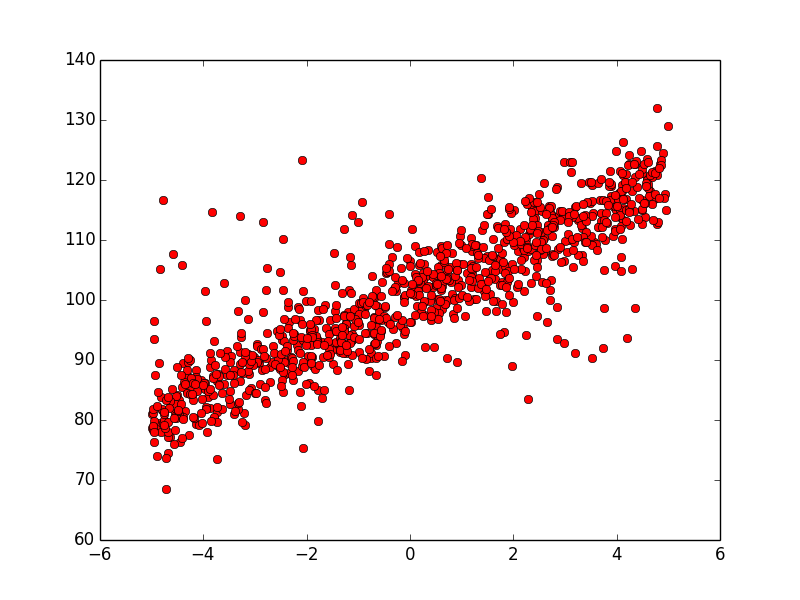
\includegraphics[width=100mm]{graphic.png}
    \caption{Вывод графика рассеяния $(y_i,x_i)$\label{overflow}}
\end{figure}
\newpage
\section{Поиск breakdown point у МНК и М-оценок}
Будем пользоваться той же моделью, как и в пункте 3.
Для поиска того процента аномальных наблюдений, при котором увеличение количества элементов выборки не повышает точности метода будем делать так:\hfill\break
\begin{itemize}
    \item Организуем цикл по процентам загрязнений $\widetilde{\varepsilon}_i$ от $\widetilde{\varepsilon}_0=0$ до $\widetilde{\varepsilon}_{100}=100$, увеличивая каждый раз $\widetilde{\varepsilon}_i$ на 1;\\
    \item На каждой итерации будем 20 раз моделировать выборку с $N_1=1000$ и $N_2=3000$ наблюдений.
    На каждой такой итерации суммируем невязку с точными значениями параметров для каждого количества элементов, а потом находим среднее, поделив на количество суммирования, т.е. посчитаем усредненную невязку:
    \begin{eqnarray}
        \widetilde{\delta}_1^{\widetilde{\varepsilon}_i}= \frac{1}{20}\sum_{k=1}^{20}(\sum_{i=0}^{n}(\beta_i-\hat{\beta}^{(N_1)}_{ki})^2)^{\frac{1}{2}},\\
        \widetilde{\delta}_2^{\widetilde{\varepsilon}_i}= \frac{1}{20}\sum_{k=1}^{20}(\sum_{i=0}^{n}(\beta_i-\hat{\beta}^{(N_2)}_{ki})^2)^{\frac{1}{2}};
    \end{eqnarray}\\
    \item если полученная усредненная невязка при 1000 наблюдений меньше либо равна невязке при 3000 наблюдений, то заканчиваем цикл - нашли breakdown point, т.е.:
            \begin{eqnarray}
                br=
                \begin{cases}
                    \widetilde{\varepsilon_i}, \textup{если}~ \widetilde{\delta}_1^{\widetilde{\varepsilon}_i}<\widetilde{\delta}_2^{\widetilde{\varepsilon}_i};
                \end{cases}
            \end{eqnarray}\\
    \item иначе повышаем процент на 1 и повторяем цикл: ~$\widetilde{\varepsilon}_{i+1}=\widetilde{\varepsilon}_{i}+0.01$
\end{itemize}
Такие тесты проведем для МНК и М-оценок.\hfill\break
\subsection{Результаты программы}
\begin{center}
\begin{tabular}{|p{8cm}|p{3cm}|}
    \hline
    \multicolumn{2}{|c|}{Найденные breakdown point для МНК и М-оценок} \\
    \hline
    Метод&breakpoint\\
    \hline
    МНК & 10\%\\
    М-оценка с функцией Хьюбера& 17\%\\
    \hline
\end{tabular}
\end{center}
Итак, видим, что М-оценки  значительно устойчивее к выбросам чем МНК, т.е.при увеличении доли аномальных наблюдений, с увеличением объема выборки, оценки не сильно изменяются.\hfill\break 
\newpage
\begin{figure}[ht!]
    \centering
    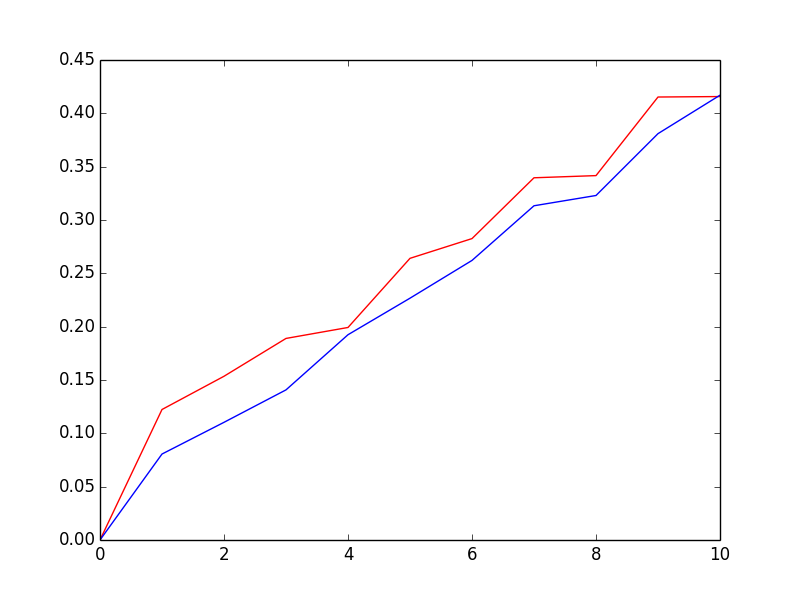
\includegraphics[width=100mm]{disperancies_MNK.png}
    \caption{График, на котором изображены $\widetilde{\delta}_1^{\widetilde{\varepsilon}_i}~\textup{красным и}~\widetilde{\delta}_2^{\widetilde{\varepsilon}_i}\textup{синим}$ относительно $\widetilde{\varepsilon_i}$\label{overflow} в случае МНК}
\end{figure}
\begin{figure}[ht!]
    \centering
    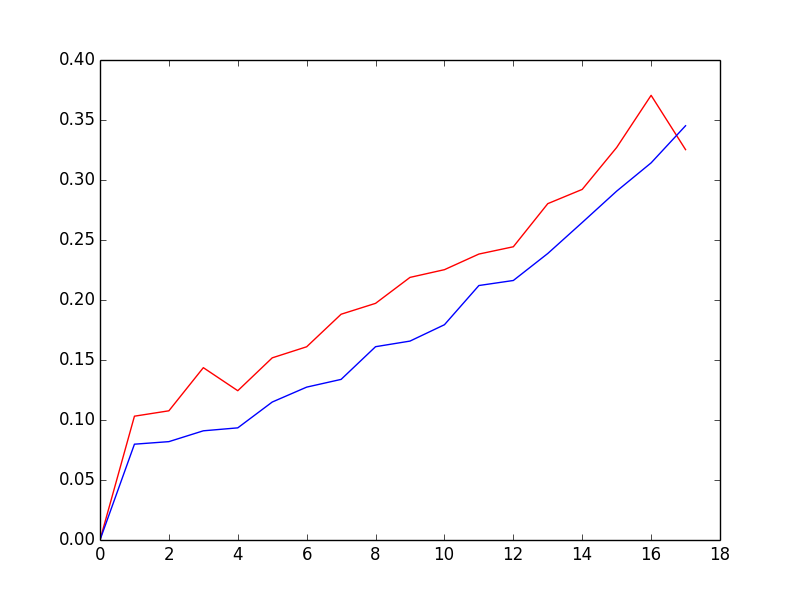
\includegraphics[width=100mm]{disperanciesMestimators.png}
    \caption{График, на котором изображены $\widetilde{\delta}_1^{\widetilde{\varepsilon}_i}~\textup{красным и}~\widetilde{\delta}_2^{\widetilde{\varepsilon}_i}\textup{синим}$ относительно $\widetilde{\varepsilon_i}$\label{overflow} в случае М-оценок}
\end{figure}
 \hfill\break
\textbf{Замечания}:
\begin{itemize}
    \item Можно моделировать не 20 раз , а значительно больше, тем самым уменьшая зависимость результата работы метода от моделируемой выборки.\\
    \item Аналогично можно заключить и для размера выборок(отношение моделируемых количеств можно значительно увеличить), однако даже для таких объемов результаты являются достаточно показательными.
\end{itemize}
\newpage
\section{Построение оценки параметров регресии с помощью группирования выборки}
Будем работать с моделью регрессии (3), предполагая что имеем регрессию без выбросов (1). 
Каждый $y_i$ принадлежит нормальному распределению:
\begin{eqnarray}
    y_i=f(x_i,\beta)+\varepsilon_i \sim \mathcal{N}(f(x_i,\beta),\sigma^2).
\end{eqnarray}
Разделим множество значений функции регрессии, т.е множество $\mathcal{R}$, на $k$ полуинтервалов:
\begin{eqnarray}
    \mathcal{R}=(-\infty,a_1]\bigcup(a_1,a_2]\bigcup \dots \bigcup(a_{k-1},+\infty ).
\end{eqnarray}
Обозначим полученные интервалы: $\nu_0,\dots,\nu_{k-1}$.\hfill\break
Далее в работе будем считать, что вместо истинных значений зависимых переменных $y_i$ наблюдается только номер класса, к которому это наблюдение попало.
Тогда для каждого $y_i$ будем набюдаем лишь номер полуинтервала $\mu_i$, в который он попал.
\begin{eqnarray}
    \mu_i=j, \textup{если $y_i$ отнесли к полуинтервалу $\nu_j$}.
\end{eqnarray}
Функцию распределения нормального закона с параметрами $\mu,\sigma^2$ можно представить как:
\begin{eqnarray}
    F(x)=\Phi(\frac{x-\mu}{\sigma}),
\end{eqnarray}
где $\Phi(x)$ функция распределения стандартного нормального закона, а $\sigma = \sqrt{\sigma^2}$:
\begin{eqnarray}
    \Phi(x)=\frac{1}{\sqrt{2}\sigma}\int_{-\infty}^{x}e^{\frac{-t^2}{2}}dt.
\end{eqnarray}
Обозначим:
\begin{eqnarray}
    \textup{erf}(x)=\frac{2}{\sqrt{\pi}}\int_0^{x}e^{-t^2}dt.
\end{eqnarray}
Тогда:
\begin{eqnarray}
    \Phi(x)= \frac{1}{2} \Big[1+\textup{erf}\Big(\frac{x}{\sqrt{2}} \Big) \Big].
\end{eqnarray}
Поэтому:
\begin{eqnarray}
    F(x)= \frac{1}{2} \Big[1+\textup{erf}\Big(\frac{x-\mu}{\sqrt{2}\sigma} \Big) \Big].
\end{eqnarray}
Тогда при модельных предположениях (15) вероятность попадания $y_i$ в полуинтервал $\nu_j$ равна:
\begin{eqnarray}
    P\{y_i\in\nu_j\}= F_{y_i}(a_{j+1})-F_{y_i}(a_{j})=
    \begin{cases}
        \frac{1}{2}(\textup{erf}(\frac{a_{j+1}-f(x_i,\beta)}{\sqrt{2}\sigma})-\textup{erf}(\frac{a_{j}-f(x_i,\beta)}{\sqrt{2}\sigma})),~j=\overline{1,k-2}\\
        \frac{1}{2}(1+\textup{erf}(\frac{a_{1}-f(x_i,\beta)}{\sqrt{2}\sigma})),~j=0\\
        \frac{1}{2}(1+\textup{erf}(\frac{a_{k-1}-f(x_i,\beta)}{\sqrt{2}\sigma})),~j=k-1
    \end{cases}.
\end{eqnarray}
Понятно, что:
\begin{eqnarray}
    P(\mu_i=j)=P(y_i\in \nu_{\mu_i}).
\end{eqnarray}
\subsection{Построение функции правдоподобия}
Составим функцию правдоподобия:
\begin{eqnarray}
    l(\beta,\sigma^2, \nu_0,\dots, \nu_{k-1})=\textup{ln}(\prod_{i=1}^{n}P(\mu_i=j))=\\
    =\sum_{i=1}^{n}\ln(P(\mu_i=j)).
\end{eqnarray}
Известно приближение для функции $\textup{erf}(x)$:
\begin{eqnarray}
    (\textup{erf} x)^2\approx 1- \exp(-x^2 \frac{\frac{4}{\pi}+ax^2}{1+ax^2}),\\
    a=\frac{8}{3\pi}\frac{3-\pi}{\pi -4}.
\end{eqnarray}
Оно считается достаточно точным для $x$ близких к $0$ и к $\infty$ \cite{Winitzki}. \hfill\break
Найдем производную для этого приближения:
\begin{eqnarray}
    \textup{erf}'(x) = \exp(-x^2 \frac{\frac{4}{\pi}+ax^2}{1+ax^2}) \frac{-2x\frac{\frac{4}{\pi}+ax^2}{1+ax^2}+(2ax^3)\frac{\frac{4}{\pi}+ax^2}{1+ax^2}-\frac{2ax^3}{1+ax^2}}{2\sqrt{1- \exp(-x^2 \frac{\frac{4}{\pi}+ax^2}{1+ax^2})}}.
\end{eqnarray}
Будем максимизировать функцию $l$.
Для этого будем искать нули ее производной. Вычисление будем производить с помощью вычислительных методов (будем использовать метод секущих), так как из-за сложного вида производной вычислить ее аналитически не представляется возможным.
\begin{eqnarray}
    \frac{\delta l}{\delta \beta}=\frac{\delta \sum_{i=1}^{n}\ln(P(\mu_i=j))}{\delta \beta}=\frac{\delta \sum_{i=1}^{n}\ln P(y_i\in \nu_{\mu_i})}{\delta \beta}=\\
    =\frac{\delta \sum_{i=1}^{n} \ln(\frac{1}{2}(\textup{erf}(\frac{a_{\mu_i+1}-f(x_i,\beta)}{\sqrt{2}\sigma})-\textup{erf}(\frac{a_{\mu_i}-f(x_i,\beta)}{\sqrt{2}\sigma})) )         }{\delta \beta}=\\
    =  \sum_{i=1}^{n}\Big((1-(\delta_{\mu_i 0}+\delta_{\mu_i k-1}))\frac{(\textup{erf'}(\frac{a_{\mu_i+1}-f(x_i,\beta)}{\sqrt{2}\sigma})-\textup{erf'}(\frac{a_{\mu_i}-f(x_i,\beta)}{\sqrt{2}\sigma}))}{ (\textup{erf}(\frac{a_{\mu_i+1}-f(x_i,\beta)}{\sqrt{2}\sigma})-\textup{erf}(\frac{a_{\mu_i}-f(x_i,\beta)}{\sqrt{2}\sigma}))}+\\
    \nonumber +(\delta_{\mu_i 0}+\delta_{\mu_i k-1})\frac{\textup{erf'}(\frac{a_{\mu_i}-f(x_i,\beta)}{\sqrt{2}\sigma})}{(1+\textup{erf}(\frac{a_{\mu_i}-f(x_i,\beta)}{\sqrt{2}\sigma}))}\Big)  (-1) \frac{\delta f(x_i,\beta)}{\delta \beta} )=\\
    =-\sum_{i=1}^{n}\begin{pmatrix}
        1\\
        x_{i1}\\
        \dots\\
        x_{in}
    \end{pmatrix}\times  \Big((1-(\delta_{\mu_i 0}+\delta_{\mu_i k-1}))\frac{(\textup{erf'}(\frac{a_{\mu_i+1}-f(x_i,\beta)}{\sqrt{2}\sigma})-\textup{erf'}(\frac{a_{\mu_i}-f(x_i,\beta)}{\sqrt{2}\sigma}))}{ (\textup{erf}(\frac{a_{\mu_i+1}-f(x_i,\beta)}{\sqrt{2}\sigma})-\textup{erf}(\frac{a_{\mu_i}-f(x_i,\beta)}{\sqrt{2}\sigma}))}+\\
    \nonumber +(\delta_{\mu_i 0}+\delta_{\mu_i k-1})\frac{\textup{erf'}(\frac{a_{\mu_i}-f(x_i,\beta)}{\sqrt{2}\sigma})}{(1+\textup{erf}(\frac{a_{\mu_i}-f(x_i,\beta)}{\sqrt{2}\sigma}))}\Big)  ,
\end{eqnarray}
где $\delta_{ij}$ - символ Кронекера.\hfill\break
Доказано, что максимизируя функцию правдоподобия (25), можем получить состоятельную оценку\cite{OLSforGrouping} параметров. \hfill\break
Итак, выражение (29) и будем использовать для метода дихотомии, приближая $\textup{erf}'(x)$ с помощью выражения (25).
\subsection{Метод секущих}
Так как мы не можем привести систему $ \frac{\delta l}{\delta \beta}=0$ к виду, удобному для итерации, то нам придется искать ее нули с помощью метода Ньютона.
Введем вектор ошибки $\check{\varepsilon}^{(k)}=\beta^{*}-\beta^{(k)}$. Тогда для его определения имеем:
\begin{eqnarray}
    \frac{\delta l (\beta^{(k)}+\check{\varepsilon}^{(k)})}{\delta \beta}=0.
\end{eqnarray}
Строя разложение левой части по формуле Тейлора и ограничиваясь лишь линейными членами\cite{NumericalMethods}, будем иметь систему:
\begin{eqnarray}
    \frac{\delta }{\delta \beta}\frac{\delta l (\beta^{(k)}}{\delta \beta}\Delta \beta^{(k)}=-\frac{\delta l (\beta^{(k)})}{\delta \beta}.
\end{eqnarray}
Если матрица $\frac{\delta }{\delta \beta}\frac{\delta l (\beta^{(k)}}{\delta \beta}$ невырожденная (а в нашем случае она диагональная), то из этой системы можно единственным образом найти $\Delta \beta^{(k)}$ и построить приближение:
\begin{eqnarray}
    \beta^{(k+1)}=\beta^{(k)}+\Delta \beta^{(k)}.
\end{eqnarray}
Так как для второй производной $l$ получится довольно сложное выражение, то будем приближать ее с помощью выражения:
\begin{eqnarray}
    \frac{\delta }{\delta \beta_j}\frac{\delta l(\beta_1^{(k)},\dots, \beta_n^{(k)}) }{\delta \beta}\approx \frac{\frac{\delta l(\beta_1^{(k)},\dots,\beta_j^{(k)},\dots, \beta_n^{(k)}) (\beta^{(k)}}{\delta \beta}-\frac{\delta l(\beta_1^{(k)},\dots,\beta_j^{(k-1)},\dots, \beta_n^{(k)}) (\beta^{(k)}}{\delta \beta}}{\beta_j^{(k)}-\beta_j^{(k-1)}}.
\end{eqnarray}
Теперь имеем нули производной функции l, а также ее значения на границе отрезка $[a,b]$.
Переберем эти значения и таким образом найдем значение вектора $\hat{\beta}$, где она достигает своего максимального значения.
% \subsection{Оценка сходимости метода секущих}
% Так как метод секущих является частным случаем метода Ньютона, то приведем теоремы




\subsection{Переклассификация выборки}
На данном этапе для каждого $x_i$ имеем класс $\mu_i$: т.е. пару $(x_i,\mu_i)$.
Теперь попытаемся переклассифицировать выборку. 
Для этом будем строить новую выборку такого же объема $N$.
Будем идти по каждому элементу $(x_i, \mu_i)$ выборки и для этого наблюдения построим новое:
\begin{equation}
    (x_i, \check{\mu}_i),
\end{equation}
где $\check{\mu}_i$ максимально встречающийся класс близлежайших соседей:
\begin{equation}
    \check{\mu}_i = \arg\max_j \sum_{|x_k-x_i|\leq \Delta,~k\neq i} \delta_{\check{\mu}_k j},
\end{equation}
где $\Delta$ параметр, задающий уровень близости. Чем он выше, тем больше используется соседей для коррекции класса нашего наблюдения.

Итак, переклассифицировав выборку, применим к ней функцию правдоподобия из уравнений (21-22), только используя теперь новые классы $\check{\mu}_i$ вместо $\mu_i$. 
Аналогично пунктам 5.1-5.2 максимизируем ее и найдем новую оценку параметров $\hat{\beta}$.

\section{Поведение производной функции правдоподобия}
На точном решении функция правдоподобия должна достигать своего максимума, а, следовательно, ее производная будет обращаться в нуль (теорема Ферма). 
С помощью этого факта и построены оценки. Теперь изучим поведение производной функции правдоподобия на точном решении до и после переклассификации выборки при разном количестве аномальных наблюдений.
Если производная функции правдоподобия на точном решении будет ближе к нулю после переклассификации выборки, значит, если мы найдем ее нуль с помощью метода, описанного в пункте 5.3, то он будет ближе к истинному решению,
 чем если бы он был найден до переклассификации выборки.
Итак, выберем такие параметры для моделирования функции регрессии:
\begin{center}
    \begin{tabular}{|p{5cm}|p{5cm}|}
        \hline
        \multicolumn{2}{|c|}{Параметры программы} \\
        \hline
        Переменная&значение\\
        \hline
        Размер выборки $N$& 500 и 1000\\
        \hline
        Доля выбросов $\widetilde{\varepsilon}$& 0.1 до 0.5\\
        \hline
        Параметры регрессии $\beta$& $(90,4)$\\
        \hline
        Регрессоры $x_i$ & $\sim U(-5,5)$\\
        \hline
        $\varepsilon_i$&$\sim N(0,15)$\\
        \hline
        $\eta_i$&$\sim N(100,100)$\\
        \hline
        $\Delta$&$1.0$\\
        \hline
        $a_2-a_1=\dots=a_{k-1}-a_{k-2}$&$0.001$\\
        \hline
        $k$&$100 000 000$\\
        \hline
    \end{tabular},
\end{center}
Итак, получили такие графики:\hfill\break
\begin{figure}[ht!]
    \centering
    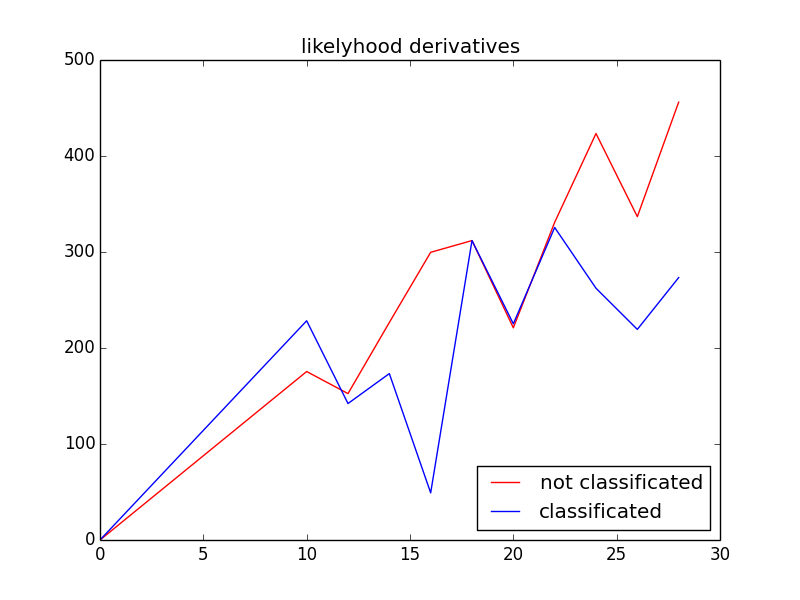
\includegraphics[width=100mm]{likelyhood_derivatives_100perc.png}
    \caption{При объеме $N=500$\label{overflow}}
\end{figure}
\newpage
\begin{figure}[ht!]
    \centering
    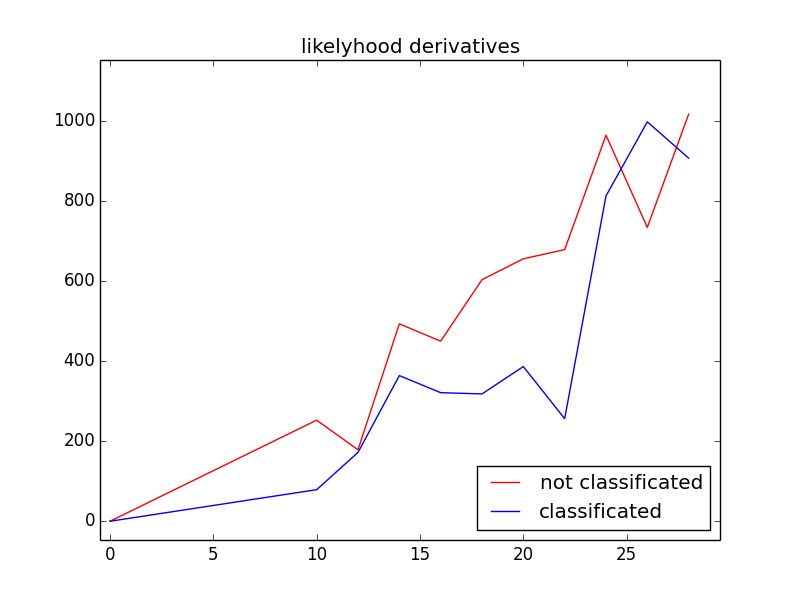
\includegraphics[width=100mm]{likelyhood_derivatives_with_1000_100perc.png}
    \caption{При объеме $N=1000$\label{overflow}}
\end{figure}
\newpage
\begin{figure}[ht!]
    \centering
    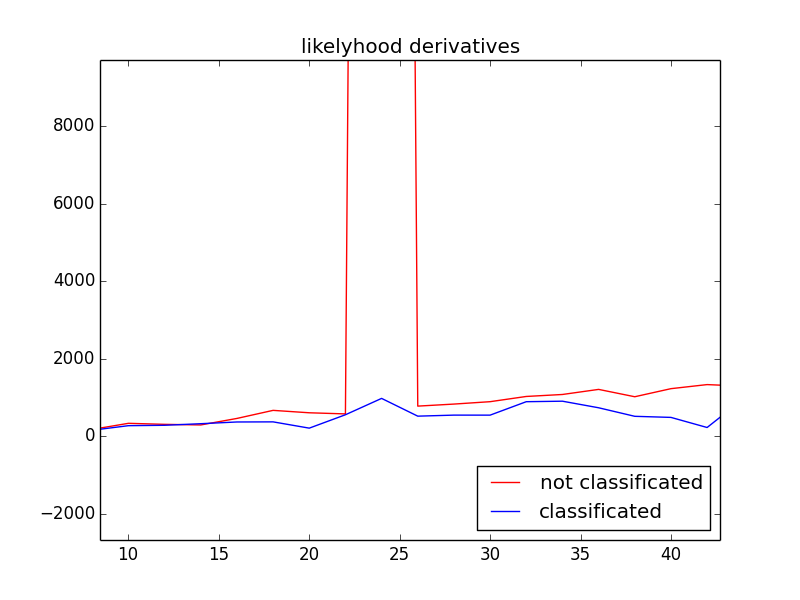
\includegraphics[width=100mm]{likelyhood_derivatives_80perc_till_50perc.png}
    \caption{При объеме $N=1000$\label{overflow}}
\end{figure}
Замечание:
\begin{itemize}
    \item Значение производной сравнительно близко к нулю, так как если взять значение, которое далеко от истинного значения параметров $\beta$, то значения производной будут на порядок выше. Например:
    \begin{eqnarray}
        \frac{\delta l(\hat{\beta})}{\delta \beta} = [ 6777.80925977~11935.60045093]^T,~\textup{при}~ \hat{\beta}= [1,1]^T,\\
        \frac{\delta l(\hat{\beta})}{\delta \beta} = [ -49.05706716~283.92412386]^T,~\textup{при}~ \hat{\beta}= [90,4]^T,\\
        \frac{\delta l(\hat{\beta})}{\delta \beta} = [-3129.555067~ -11908.91415502]^T,~\textup{при}~ \hat{\beta}= [170,8]^T.
    \end{eqnarray}
\end{itemize}
\section{Заключение}
Были описаны некоторые методы робастного оценивания параметров регрессии.
В курсовой работе был предложен еще один способ оценки ``меры робастности'' ~методов: \textit{``breakdown point''}, который был далее использован на описанных методах оценивания --- М-оценках и МНК.
Был предложен еще один способ оценивания параметров регрессии для модели регрессии с аномальными наблюдениями при наличии группирования выборки. 
С проведением вычислительного эксперимента было исследовано поведение производной функции правдопобия на точном решении для метода, описанного в пункте 5.
\newpage
% \section{Список литературы}
% \printbibliography
\begin{thebibliography}{9}
    \bibitem{Huber}
    Хьюбер Дж П.,
    \textit{Робастность в статистике:пер. с англ.}.
    М.:Мир,1984-304с

    \bibitem{Kharin}
    Харин Ю.С., Зуев Н.М.,
    Жук Е.Е,
    \textit{Теория вероятностей, математическая и прикладная статистика: учебник}
    Минск: БГУ, 2011.-463с

    \bibitem{RobustRegression}
    John Fox \& Sanford Weisberg,
    \textit{Robust Regression},
    October 8, 2013

    \bibitem{RobustPolynomialEstimation}
    А.В. Омельченко,
    \textit{Робастное оценивание параметров полиномиальной регрессии второго порядка,}
    Харьковский национальный университет радиоэлектроники, Украина, 2009

    \bibitem{ComparisonRobust}
    \"{O}zlem G\"{u}r\"{u}nl\"{u} Alma,
    \textit{Comparison of Robust Regression Methods
    in Linear Regression},
    Int. J. Contemp. Math. Sciences, Vol. 6, 2011, no. 9, 409 - 421

    \bibitem{Winitzki}
    Sergei Winitzki,
    \textit{A handy approximation for the error function and its inverse}

    \bibitem{NumericalMethods}
    Мандрик П.А., Репников В.И., Фалейчик Б.В.,
    \textit{Численные методы}

    \bibitem{OLSforGrouping}
    Е. С Агеева, чл.-корр. НАН Беларуси Ю.С. Харин,
    \textit{Состоятельность оценки максимального правдопобия параметров множественной регрессии по классифицированным наблюдениям}
\end{thebibliography}
\addcontentsline{toc}{section}{Список Литературы}
\end{document}